\documentclass{article}
\usepackage[pdfcreator={LaTeX}]{hyperref}
\usepackage{graphicx}
\usepackage[utf8]{inputenc} 
\usepackage[ngerman]{babel}


\usepackage{tikz}
\usetikzlibrary{arrows,shadows}
\usepackage{pgf-umlsd}


\begin{document}
\begin{titlepage}

\begin{center}
\textbf{\textsc{\LARGE Entwurf}}

{\large \today}

\vspace{2cm}
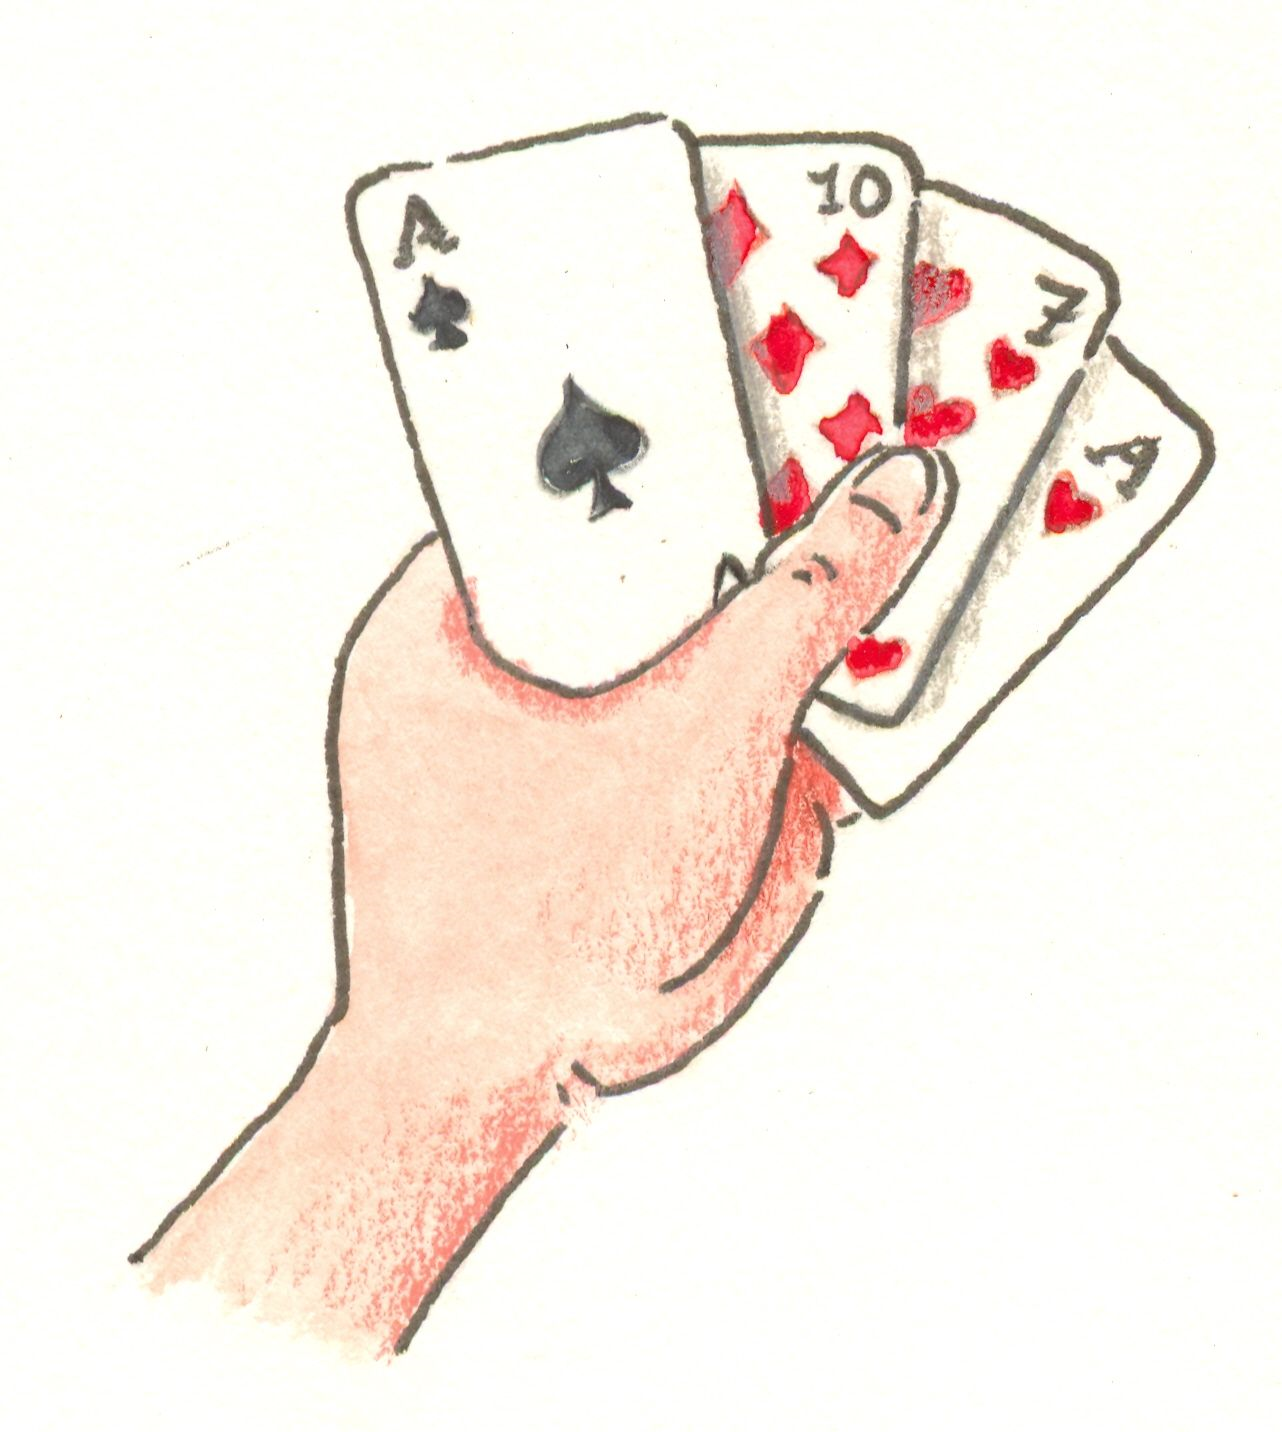
\includegraphics{kartenspiel}
\ \\
\ \\

\textbf{\textsc{\LARGE NET-WizHearts}}
\vspace{2cm}

\begin{tabular}{|c|c|c|}\hline
   Phase & Verantwortlicher & E-Mail \\ \hline\hline
   Pflichtenheft & Alina  Meixl  &  alina@meixl.de \\ \hline
   Entwurf & Viktoria Witka & witkaviktoria@freenet.de \\ \hline
   Spezifikation & Daniel Riedl & dariedl14@yahoo.de \\ \hline
   Implementation & Andreas Altenbuchner& a.andi007@gmail.com\\ \hline
   Verifikation &Patrick Kubin & kubin@fim.uni-passau.de\\ \hline
   Präsentation & w& w\\ \hline
 \end{tabular}

\end{center}

\end{titlepage}


\tableofcontents
\newpage

\section{Einleitung}
-----Achtung Kopie -------
In diesem Dokument wird der konzeptionelle Entwurf des Online Multiplayer Kartenspiels NET-WizHearts dargestellt.\\
\ \\
Es wird eine erste Übersicht über die verschiedenen Komponenten des MVC-
Modells, das der Anwendung zugrunde liegt, gegeben. Dies geschieht durch eine
Angabe der Klassenstruktur. Einzelne Funktionsaufrufe
werden beispielhaft zu Illustrationszwecken in Sequenzdiagrammen dargestellt.\\
\ \\
Durch das Verwenden des MVC Design Patterns wird eine Unabhängigkeit der View-Schicht 
vom restlichen System erzielt, so dass die graphisch Oberfläche - wie gefordert - ohne Anpassung 
der Modell- und Controllerschicht auch für andere Regelwerke einsetzbar ist.\\
\  \\
WEITERES


\section{Architektur-Diagramm}
Client-Server Diagramm. Client hat MVC Architektur.
\  \\
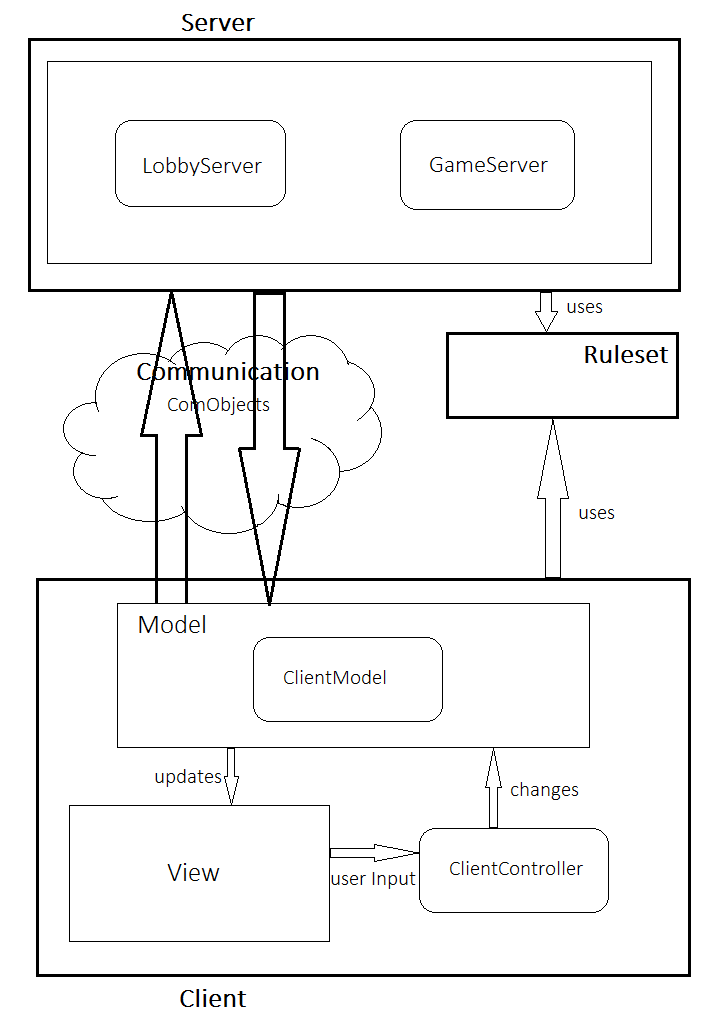
\includegraphics[height=15cm]{ArchitekturDiagramm}
\newpage
\section{Klassendiagramm}
\subsection{Packages}
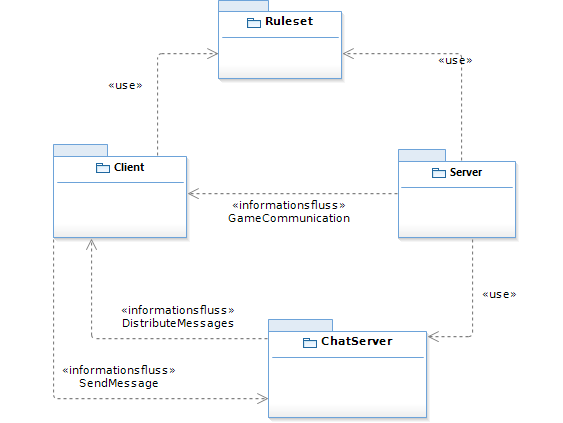
\includegraphics[width=\textwidth]{Packages}
\subsection{Server}
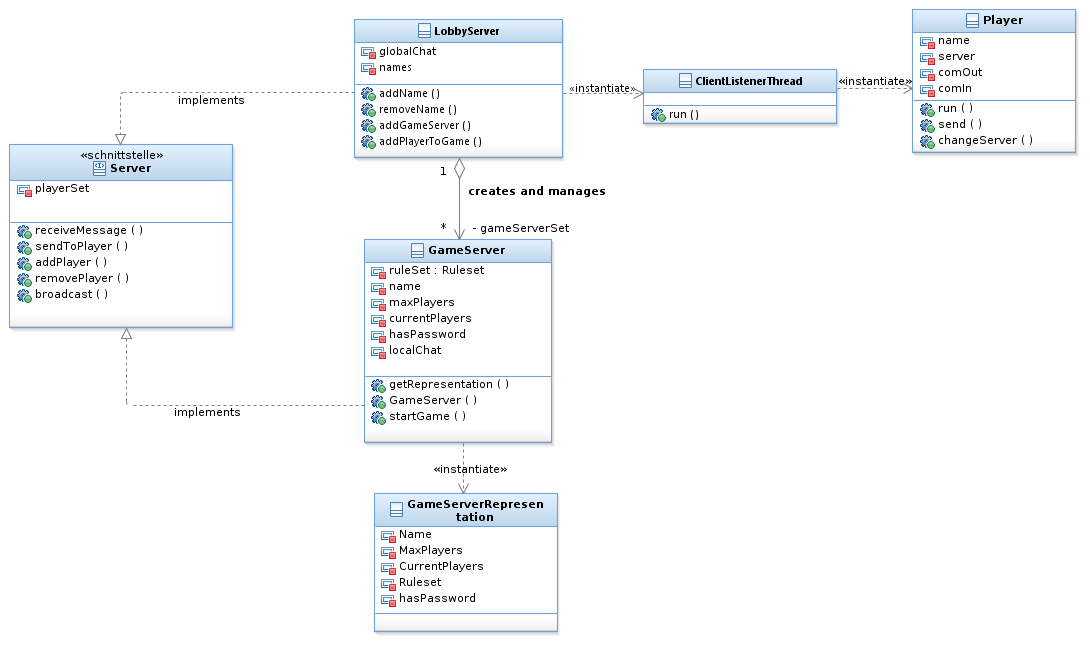
\includegraphics[width=\textwidth]{Server}
\subsection{Client}
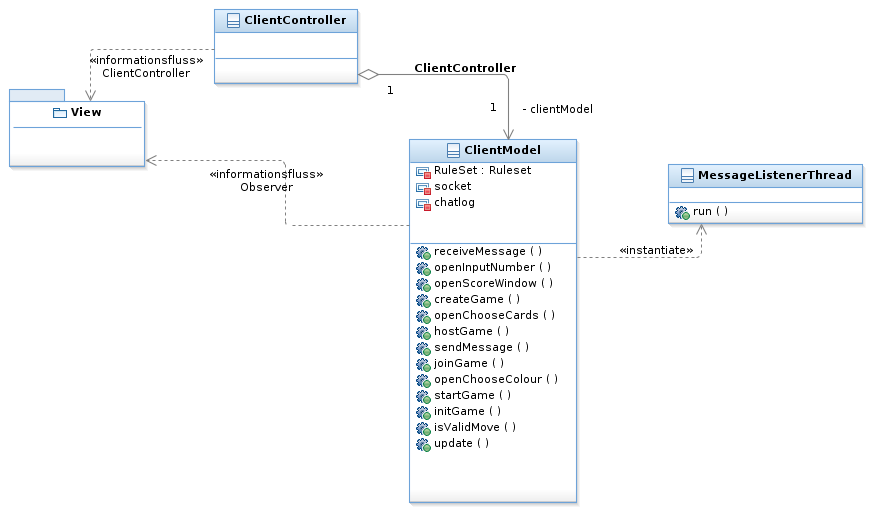
\includegraphics[width=\textwidth]{Client}
\subsection{ClientView}
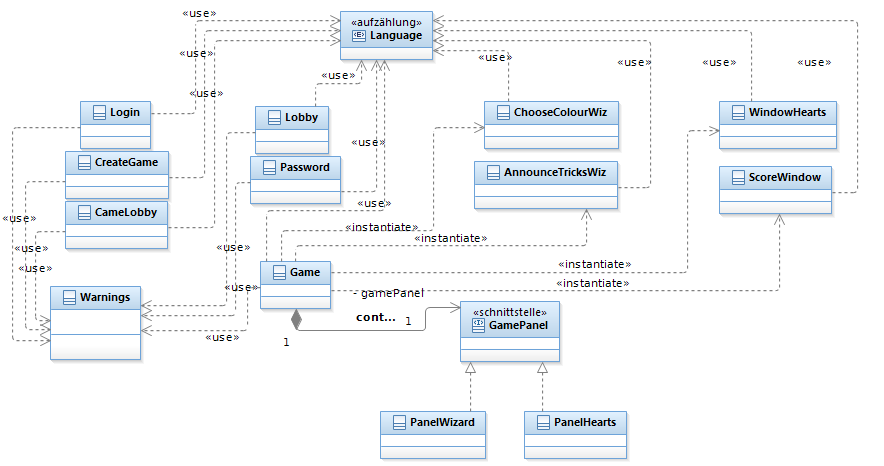
\includegraphics[width=\textwidth]{ClientView}
\subsection{Ruleset}
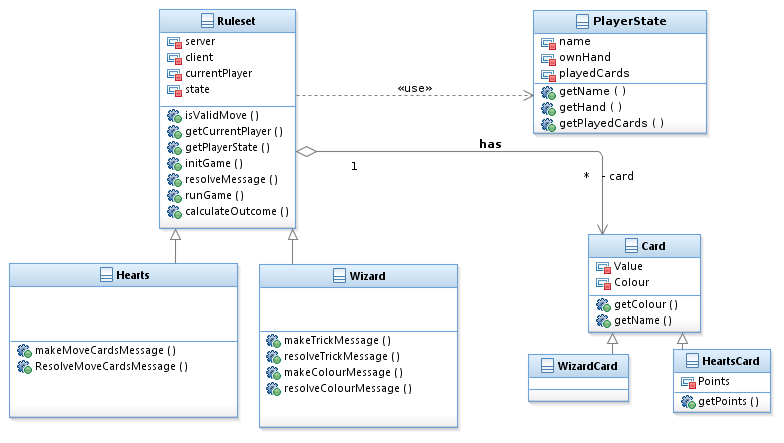
\includegraphics[width=\textwidth]{Ruleset}

\ \\
\section{Klassenbeschreibung}
Wichtigste Klassen und ihr Verwendungszweck.
	\subsection{Server}
		\textbf{ServerMain} ist die Hauptklasse des Servers welche Konfiguration und Wartung des Servers implementiert. \\
		\textbf{Schnittstelle Server} liefert einen Satz von Methoden die von der LobbyServer-Klasse und der GameServer-Klasse implementiert werden. \\
		Mit receiveMessage() kann eine Playerinstanz ein ComObjekt an eine Serverinstanz zur weiteren Verarbeitung weiterleiten. \\
		Mit sendToPlayer() kann eine Serverinstanz ein ComObjekt an eine Playerinstanz weiterreichen. \\
		Sammelaufrufe werden durch die broadCast() Methode implementiert.
		\textbf{LobbyServer} erstellt neue Spiele (/F126/) und ist sowohl für die Verwaltung aller Spiele (/L110/), als auch der Spieler in der Lobby zuständig (/L100/). Die LobbyServer-Klasse implementiert die Server-Schnittstelle. Über die Methode addGameServer() wird ein Spiel erstellt (/L300/) und addPlayerToGame() fügt Spieler bestehenden Spielen hinzu. Es werden auflaufende ComObjekte anhand ihrer Klasse weiterverarbeitet und steuern so die Belange der Lobby. \\
		\textbf{ClientListenerThread} akzeptiert eingehende TCP-Verbindungen und erstellt instanzen der Klasse Player. \\
		\textbf{GameServer} verwaltet ein Spiel, dessen Spieler, sowie den Chatroom im Spiel (/L260/). Der GameServer leitet Aufrufe vom Regelwerk an die betreffenden Spieler weiter. Die GameServer-Klasse implementiert die Server-Schnittstelle. Über den Methodenaufruf startGame() können Spiele vom Spielleiter gestartet werden. Es werden auflaufende ComObjekte anhand ihrer Klasse weiterverarbeitet und steuern so die Belange des Spieles.\\
		\textbf{Player} repräsentiert einen Client, enthält den Namen des Clients und verwaltet die Ein- und Ausgänge seiner Socketverbindung. Send() ermöglicht es Serverinstanzen-ComObjekte an den Client zu senden. \\
	\subsection{Ruleset}
		\textbf{Ruleset} ist eine abstrakte Klasse welches zu einem Spiel die Regeln und den Ablauf bestimmt (/L280/). Außerdem überprüft es ob jeder neuer Spielzustand regelkonform ist (/L280/). Das Regelwerk wird im Client, sowie im Server instanziert. Im Server hält es Zustandsinformationen von allen Spielern, im Client jedoch nur von seinem entsprechendem Spieler (/L330/). Über resolveMessage() kann eine GameServerinstanz ein ComObjekt von Player an das Regelwerk weiterleiten. Die Methoden runGame() und calculateOutcome() starten das Spiel bzw ermitteln den Gewinner und Punktestand eines Spiels. \\
		\textbf{Hearts} erbt von Ruleset und erstellt das Regelwerk zum Spiel Hearts. \\
		\textbf{Wizard} erbt von Ruleset und erstellt das Regelwerk zum Spiel Wizard. \\
		\textbf{PlayerState} modelliert den Spielzustand eines Spielers, dessen Namen, Karten und Spielzug. Auch hält die Klasse die dazugehörigen getter Methoden bereit. PlayerState wird von Instanzen des Ruleset verwendet. \\
		\textbf{Card} ist eine abstrakte Klasse und repräsentiert eine Karte. Jede Karte besitzt als Attribute einen Wert und eine Farbe. \\
		\textbf{HeartsCard} repräsentiert eine Karte aus dem Spiel Hearts. \\
		\textbf{WizardCard} repräsentiert eine Karte aus dem Spiel Wizard.
	\subsection{ComObjects}
		\textbf{ComObject} Grundlegende ComObject Klasse von der alle anderen erben.\\
		\textbf{ComInitLobby} Synchronisiert den Client mit der Lobby wenn er sich mit dem Server verbindet oder nach einem Spiel in die Lobby zurückkehrt. \\
		\textbf{ComUpdatePlayerList} \\
		\textbf{ComLogin} Nachricht die beim Login an den Server gesendet wird.\\
		\textbf{ComLobbyUpdateGameList} Aktualisiert die Spielerliste in der Lobby und Spiellobby.\\
		\textbf{ComInitGameLobby} Liefert die Liste der Spieler die sich bereits beim Betreten der Spiellobby darin befinden. \\
		\textbf{ComChatMessage} Das ComObjekt einer Chatnachricht. Liefert die Chatnachricht in Form eines Strings.\\
		\textbf{ComRuleset} Grundlegende Nachricht eines Regelwerkaufrufes. Trägt eine verfeinerte Nachricht mit weiteren Informationen.\\
		\textbf{RulesetMessage} vererbt an alle Nachrichten für das Regelwerk.\\
		\textbf{MsgCard} Beinhaltet die ausgespielte Karte eines Spielers.\\
		\textbf{MsgNumber} Gibt eine Nummer zurück, welche für die Stichansage in Wizard verwendet werden kann.\\
		\textbf{MsgSelection} Gibt eine Farbe zurück, welche für die Ansage der Trumpfarbe in Wizard verwendet werden kann.\\
		\textbf{MsgMultiCards} Liefert mehrere Karten zum Tausch für das Regelwerk Hearts. \\
		\textbf{MsgUserInputRequest} Wird dem Client gesendet um den aktuellen Zug anzusagen.\\
		\textbf{enum commands}  Enumerator der ComObjekte ihre Kommandos zuweist. \\
		\textbf{enum types} Enumerator zur eindeutigen Identifizierung von Regelwerknachrichten.
	\subsection{Client}
	\subsubsection{Model}
		\textbf{MessageListenerThread} wird von dem ClientModel instanziert und hält die TCP-Verbindung zum Server. Der Thread tauscht ComObjekte mit dem Server aus und greift über die receiveMessage() Methode auf das ClientModel zu.
		\textbf{ClientModel} ist die Schnittstelle zwischen dem MessageListenerThread, dem Ruleset und der View. Das Model prüft Nachrichten und leitet Kommandos aufgrund ihrer Klasse an das Regelwerk oder die GUI weiter. Mit receiveMessage() kann der Klasse ein ComObjekt übergeben werden. Über sendMessage() können Kommandos vom Regelwerk oder der GUI an den Server gesendet werden.
		
	\subsubsection{Controller}
	\subsubsection{View}
			\textbf{Language} ist ein Enumerator der von Komponenten der View zur Darstellung unterschiedlicher Sprachen verwendet wird (/L350W/). \\
			\textbf{Login} repräsentiert den initialen Dialog indem der Benutzer seinen Namen (/F042/) und die Adresse des Servers (/F040/) eingeben kann. Außerdem ist über den Login die Auswahl der Sprache möglich (/F050W/). Über den Login wird ebenfalls die Verbindung zum Server hergestellt (/F045/).\\
			\textbf{Lobby} erzeugt die Ansicht der ServerLobby. Es können offene Spiele (/L110/) und Spieler (/L100/) betrachtet sowie Chatnachrichten gesendet (/F060/) und empfangen werden (/L115/). Über Leave verlässt der Spieler das Spiel (/F090/). Über Host Game (/F080/) wird der Spieler zum CreateGame Fenster weitergeleitet und mit Join Game (/F070/) kann einem bereits erstelltem Spiel beigetreten werden. \\
			\textbf{CreateGame} bietet alle Komponenten um ein Regelwerk zu wählen (/F120/), einen Spielnamen fest zulegen (/F122/) und das Spiel durch ein Passwort zu schützen (/F130W/). In der Spielerstellung wird ein Titelbild des ausgewähltem Spiels und eine kurze Beschreibung angezeigt (/L120/, /L122/). Über Leave kehrt der Spieler in die Lobby zurück (/F124/) und mit Create wird das Spiel erstellt (/F126/).\\
			\textbf{Password} ermöglicht die Eingabe eines Passwortes (/F140W/) um einem geschlossenem Spiel beizutreten (/F142/) oder  per Leave wieder in die Lobby zurückzukehren (/F145/). \\
			\textbf{GameLobby} modelliert das Wartefenster indem beigetretene Spieler (/L155/) auf den Start des Spieles durch den Spielleiter warten (/F200/). Der Spielleiter kann Spieler mit dem Remove Player Button entfernen (/F180/). Über Leave kehren die Spieler in die Lobby zurück (/F170/) und (/F190/). Der spielinterne Chat ist ab hier verfügbar (/F160/) und (/L158/). \\
			\textbf{Game} ist der allgemeine Teil des Spielfensters der den Spielchat beherbergt (/F220/) und (/L260/). Schließen beendet das Spiel und der Spieler wird in die Lobby zurückgeleitet (F210/). Alle Spielfenster zeigen die eigenen Karten (/L190/), sowie zum Ausspielen anwählbare Karten (/F225/) und (/F230/). Die Anzahl der Karten der Mitspieler (/L192/) und den Ablagestapel (/L194/). Nach jeder Runde wird der Punktestand  aktualisiert (/L200/).\\
			\textbf{PanelWizard} ist die für das Spiel Wizards angepasste Teilkomponente des Spielfensters.  \\
			\textbf{PanelHearts} ist die für das Spiel Hearts angepasste Teilkomponente des Spielfensters. \\
			\textbf{Warning} gibt Fehlermeldungen und Hinweise aus (/L290/). \\
			\textbf{ChooseColour} ermöglicht es Spielern in einer Partie Wizards die Trumpffarbe auszuwählen (/F360/). \\
			\textbf{InputNumber} erstellt ein Fenster, über das man zu Beginn einer Runde Wizards seine Stiche tippen kann (/F370/). \\
			\textbf{ChooseCards} erzeugt ein Fenster zu beginn einer Partie Hearts über das Karten zu anderen Spielern weitergereicht werden müssen (/F260/). \\
			\textbf{ScoreWindow} zeigt den Punktestand nach einem Spiel oder Runde an (/L250/).\\

\section{Sequenzdiagramme}
	\subsection{Spielstart}
		Mr. Blue, Mr. White und Mr.Pink befinden sich in der Lobby. \\
		Mr. Blue klickt auf 'New Game' und wird ins Erstellungsfenster geschickt. \\
		Er nimmt die nötigen Einstellungen vor(z.B Wizard auswahlen, Name setzen) und druckt auf 'Create'. Er wird ins  Wartefenster weitergeleitet.\\
		Mr. Pink und Mr. White wählen Mr. Blues spiel in der Lobby aus und drücken auf 'Join'. Sie werden an die Passwortabfrage geschickt.\\
		Sie geben das Passwort ein und werden ans Wartefenster geschickt.\\
		Die Mindestanzahl von drei ist erreicht. Mr. Blue drückt auf 'Start Game'.\\
		Mr. Blue, Mr. Pink und Mr. White werden ins Spiel geschickt. Das Spiel startet.\\


\newpage
\setlength{\hoffset}{-30mm}
\setlength{\topmargin}{-3.0cm}
\begin{sequencediagram}

\newthread[white]{b}{B}
\newinst[0.1]{w}{W}
\newinst[0.1]{p}{P}
\newinst[0.1]{l}{Lobby}
\newinst[0.1]{e}{CreateG.}
\newinst[0.1]{g}{GLobby}
\newinst[0.1]{a}{Game}
\newinst[0.1]{c}{CModel}
\newinst[0.1]{s}{Server}
\newinst[0.1]{gs}{GServer}

\mess{b}{klicknewGame}{l}	
\begin{call}{l}{newGame()}{c}{}
	\begin{call}{c}{close()---Lobby Mr.Blue}{l}{}	
	\end{call}	
	\mess{c}{toCrGameMrBlue}{s}	
	\mess{s}{removePlayerMrBlue}{c}			
	\begin{call}{c}{removePlayer(Mr.Blue)}{l}{}	
	\end{call}
	\begin{call}{c}{open()--- Mr.Blue}{e}{}
		\mess{b}{RulesetWizard,Name,Create}{e}
		\begin{call}{e}{openGame()}{c}{}	
		\end{call}		
	\end{call}
	\begin{call}{c}{close()}{e}{}	
	\end{call}
	\begin{call}{c}{open()--- Mr.Blue}{g}{}
			\mess{c}{newGameMrBlue}{s}
			\begin{call}{s}{newGameServer(Mr.Blue,Wizard, 'MrBluesGame')}{gs}{}				
				\mess{s}{openedGameMrBlue}{c}
				\begin{call}{c}{addOpenedGame(Mr.BluesGame, Wizard)}{l}{}
					\mess{b}{Hier 2te Seite}{l}
				\end{call}
			\end{call}
		\end{call}	
\end{call}	

\end{sequencediagram}
\newpage
\setlength{\hoffset}{0mm}
\setlength{\topmargin}{0cm}
	
\newpage
\setlength{\hoffset}{-30mm}
\setlength{\topmargin}{-3.0cm}
\begin{sequencediagram}

\newthread[white]{b}{B}
\newinst[0.1]{w}{W}
\newinst[0.1]{p}{P}
\newinst[0.1]{l}{Lobby}
\newinst[0.1]{e}{CreateG.}
\newinst[0.1]{g}{GLobby}
\newinst[0.1]{a}{Game}
\newinst[0.1]{c}{CModel}
\newinst[0.1]{s}{Server}
\newinst[0.1]{gs}{GServer}
\mess{w}{klickOpenGameMrBluesGame}{l}
	\begin{call}{l}{joinGame(MrWhite)}{c}{}
		\begin{call}{c}{close()---Lobby Mr.White}{l}{}	
		\end{call}	
		\mess{c}{WjoinMrBlue}{s}	
		\begin{call}{s}{addToPlayer(Mr.White)}{gs}{}	
		\end{call}
		\mess{s}{removePlayerMrWhite}{c}
		\begin{call}{c}{removePlayer(Mr.White)}{l}{}	
		\end{call}
		\begin{call}{c}{join()--- Mr.White}{g}{}
		\end{call}
	\end{call}
\mess{p}{klickOpenGameMrBluesGame}{l}
	\begin{call}{l}{joinGame(MrPink)}{c}{}
		\begin{call}{c}{close()---Lobby Mr.Pink}{l}{}	
		\end{call}	
		\mess{c}{WjoinMrBlue}{s}	
		\begin{call}{s}{addToPlayer(Mr.Pink)}{gs}{}	
		\end{call}
		\mess{s}{removePlayerMrPink}{c}
		\begin{call}{c}{removePlayer(Mr.Pink)}{l}{}	
		\end{call}
		\begin{call}{c}{join()--- Mr.Pink}{g}{}
		\end{call}
	\end{call}
	\mess{b}{startGame}{g}
	\begin{call}{g}{goToGame()}{c}{}
	\end{call}
	\begin{call}{c}{close()}{g}{}	
	\end{call}
	\begin{call}{c}{open()}{a}{}
	\end{call}

\end{sequencediagram}
\newpage
\setlength{\hoffset}{0mm}
\setlength{\topmargin}{0cm}


	\subsection{Spielzug}
		Aufgabe: Ein Spieler ist im Spiel Wizard an der Reihe und spielt eine Karte aus.
		Das Diagramm endet sobald der Spielzug auf allen Clients sichtbar
		geworden ist und der nächste Spieler seinen Zug machen kann.\\
		\ \\
		Mr. Blue, Mr. White und Mr.Pink sind im Spiel Wizard. \\
		Mr. Blue ist an der Reihe, wahlt eine Karte durch einmaliges anklicken aus und spielt sie durch ein weiteres anklicken.\\
		Der Zug wird auf Regelkonformität überprüft.\\
		Er ist nicht regelwidrig, also wird die gepielte Karte über den Server verschickt und bei Mr. Blue, Mr. Pink und Mr. White auf dem 	Ablagestapel angezeigt. \\
		Es wird überpruft, wer als nächstes dran ist.\\
		Der nächste Spieler ist am Zug \\

\newpage
\setlength{\hoffset}{-30mm}
\setlength{\topmargin}{-3.0cm}
\begin{sequencediagram}
\newthread[white]{b}{Mr.B}
\newinst[0.3]{g}{Bs Game}
\newinst[0.3]{w}{Ws Game}
\newinst[0.3]{p}{Mr. Ps Game}
\newinst[0.3]{c}{ClientCon.}
\newinst[0.3]{m}{ClientMod}
\newinst[0.3]{rc}{RWClient}
\newinst[0.3]{gs}{GServer}
\newinst[0.3]{rs}{RWServer}

\mess{b}{klickCardTwice}{g}
\begin{call}{g}{playCard()}{c}{}
	\begin{call}{c}{checkRulesLocal(Card)}{m}{true}
		\begin{call}{m}{checkRulesLocal(Card)}{rc}{true}
		\end{call}
	\end{call}
	\begin{call}{m}{checkRulesGlobal(Card)}{gs}{true}
		\begin{call}{gs}{checkRulesGlobal(Card)}{rs}{true}
		\end{call}
	\end{call}

	\begin{call}{gs}{playedCard(Card)}{m}{}
		\begin{call}{m}{update()}{g}{}
		\end{call}
		\begin{call}{m}{update()}{w}{}
		\end{call}
		\begin{call}{m}{update()}{p}{}
		\end{call}
	\end{call}

	\begin{call}{m}{checkNextPlayer()}{m}{}
	\end{call}
	\begin{call}{m}{notifyNextPlayer()}{w}{}
	\end{call}
\end{call}

\end{sequencediagram}
\newpage
\setlength{\hoffset}{0mm}
\setlength{\topmargin}{0cm}			
\end{document}
